\documentclass[14pt]{extarticle}

\usepackage{geometry}
\usepackage{amsmath,amsthm,amssymb}
\usepackage[utf8]{inputenc}
\usepackage[T1,T2A]{fontenc}
\usepackage{bold-extra}
\usepackage[english,russian]{babel}
\usepackage{indentfirst}
\usepackage{graphicx}
\graphicspath{ {images/} }
\usepackage{float}
\usepackage{listings}
\usepackage{lmodern}
\usepackage{appendix}
\usepackage{braket}
\usepackage{cite}
\usepackage[nottoc,numbib]{tocbibind}

\geometry{
a4paper,
left = 20mm,
right = 15mm,
bottom = 20mm,
top = 20mm,
}
\renewcommand{\rmdefault}{ftm} % TimesNewRoman
\renewcommand{\baselinestretch}{1.5} 

\begin{document}

\begin{titlepage}
	\begin{center}
		\small{ФЕДЕРАЛЬНОЕ ГОСУДАРСТВЕННОЕ БЮДЖЕТНОЕ ОБРАЗОВАТЕЛЬНОЕ}\\ 
			УЧРЕЖДЕНИЕ ВЫСШЕГО ОБРАЗОВАНИЯ\\
			«МОСКОВСКИЙ ГОСУДАРСТВЕННЫЙ УНИВЕРСИТЕТ\\
			имени М.В.ЛОМОНОСОВА»\\
		\hfill \break
		ФАКУЛЬТЕТ ВЫЧИСЛИТЕЛЬНОЙ МАТЕМАТИКИ И КИБЕРНЕТИКИ\\
		КАФЕДРА СУПЕРКОМПЬЮТЕРОВ И КВАНТОВОЙ ИНФОРМАТИКИ\\
		\vfill
		ЗАДАНИЕ 1 \\
		\textbf{<<РАСПИСАНИЕ СЕТИ СОРТИРОВКИ>>}\\
		КУРСА \\
		\textbf{<<ПАРАЛЛЕЛЬНЫЕ ВЫЧИСЛЕНИЯ>>}\\
	\end{center}	
	\vfill
	\begin{flushright}
		Выполнил студент группы м118:\\
		Пухов Д. Н.\\
		Дата подачи: 28.02.2018
		%{\hspace{3cm}}
		\vfill
	\end{flushright}
	
	
	\begin{center}
		Москва \\
		2018
	\end{center}
	
	\thispagestyle{empty}

\end{titlepage}

\tableofcontents
\newpage



\section{Формулировка задачи}
Разработать последовательную программу вычисления расписания сети сортировки, числа использованных компараторов и числа тактов, необходимых для её срабатывания при выполнении на $n$ процессорах. Число тактов сортировки при параллельной обработке не должно превышать числа тактов, затрачиваемых чётно-нечётной сортировкой Бетчера.

\section{Алгоритм решения}
Решение задачи состоит их двух действий: выбрать сеть сортировки и построить её расписание.
Наиболее очевидное решение первой проблемы --- использовать обменную сортировку слиянием Бэтчера (т.е. чётно-нечётную сортировку Бэтчера), поскольку эта сортировка удовлетворяет ограничению на число тактов (здесь такт ---- единица измерения времени, не относящаяся к процессору напрямую). Недостаток данной сети в том, что она не является самой быстрой. С другой стороны, эта сеть масштабируется на произвольное число процессоров, в то время как алгоритм построения самой быстрой сети сортировки для произвольного числа процессоров в настоящее время неизвестен.

\subsection{Описание сети Бэтчера}
Сеть сортировки, основанная на слиянии Бэтчера, по построению неотличима от обычной сортировки слиянием:
\begin{lstlisting}
sort(array):
	if array length < 2  return
	sort(left half of array)
	sort(right half of array)
	merge(left half of array, right half of array)
\end{lstlisting}

Рассмотрим главную часть алгоритма --- слияние.
Пусть на входе имеются две отсортированных последовательности: $x_1, x_2, ..., x_n$ и $y_1, y_2, ..., y_m$ с произвольным числом элементов $n$ и $m$. После слияния мы должны получить отсортированную последовательность длины $n+m$. Очевидно, при $n \cdot m = 0$ действий выполнять не требуется. При $n \cdot m = 1$ требуется ровно один компаратор. В случае $n \cdot m > 1$ нужно произвести слияние нечётных элементов первой и второй последовательностей, слияние чётных элементов первой и второй последовательностей и затем в получившейся последовательности $v_1, v_2, ..., v_{m+n}$ упорядочить с помощью компараторов пары $2:3, 4:5, ..., (m+n-1):(m+n)$. Доказательство основывается на принципе нулей и единиц и здесь не рассматривается (см. Д.Кнут, Сортировка и поиск). Ниже изображена сортировка для 15 элементов в случае последоватлельного выполенения (нумерация с 0, отрицательные ординаты стоит воспринимать по абсолютной величине как номера процессоров). По оси абсцисс отложены такты --- время выполнения сортировки. Можно видеть, что сначала массив разбивается на 8 (вверху) и 7 (внизу) элементов, затем 8 элементов разбиваются на 4 и 4, затем 4 разбиваются на 2 и 2, 2 на 1 и 1, после чего начинается слияние в обратном порядке.

Здесь же можно заметить, что при выполнении сортировки на 15 процессорах (у каждого процессора по одному элементу) многие сравнения-обмены могут выполняться одновременно. Например, на первом такте могут быть выполнены следующие сравнения-обмены: 0:1, 2:3, 4:5, 6:7, 8:9, 10:11, 12:13. А взаимодействие 1:3, к примеру, не может быть вполнено на первом такте, процессор 1 на первом такте занят (и процессор 3 занят, что в данном случае неважно). Таким образом, при параллельной сортировке время работы будет меньше, чем при последовательной. Для 15 процессоров получим 10 тактов против 59.

\begin{figure}[H]
	\centering
	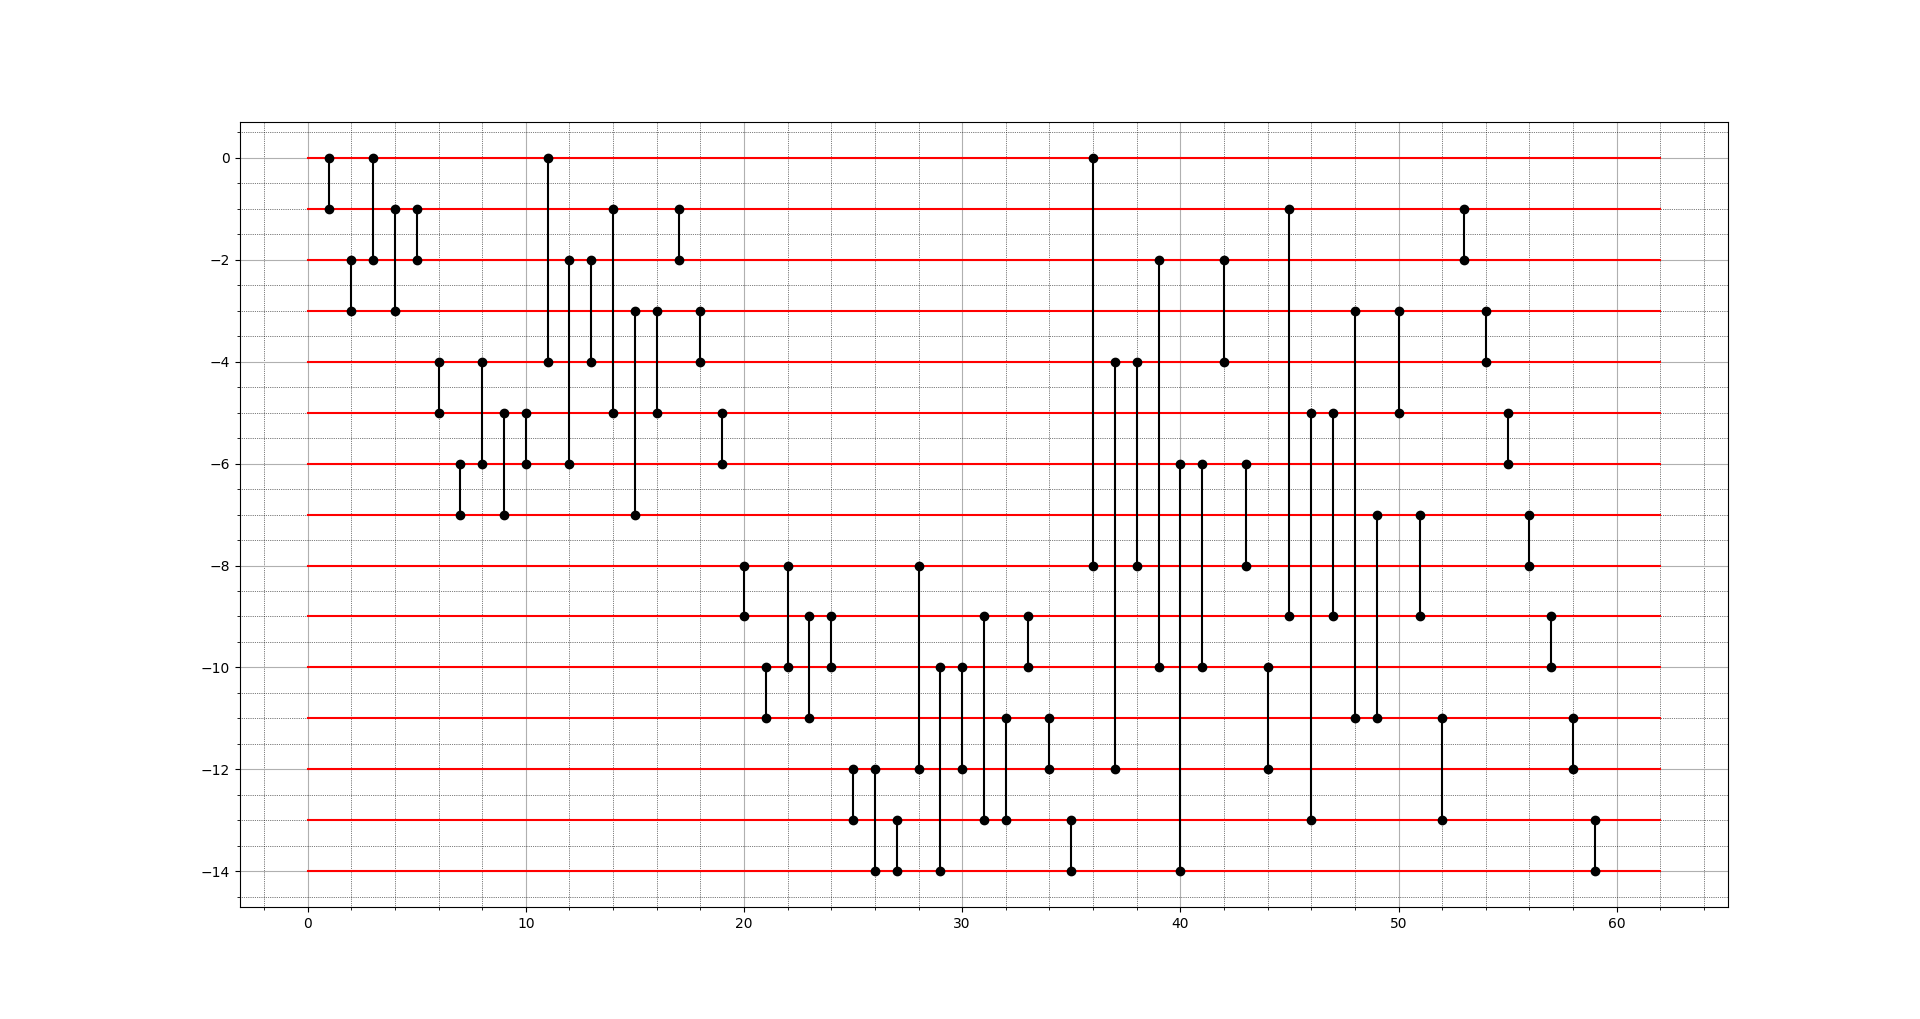
\includegraphics[scale=0.4]{network}
	\caption{Сеть обменной сортировки со слиянием Бэтчера для 15 элементов}
\end{figure}

\subsection{Построение сети на одном процессоре}
Сеть будем строить исходя из определения --- т.е. тоже рекурсивно. 
Заметим, что функция сортировки, разделяющая массив на две части (верхнюю и нижнюю), требует ровно два параметра: номер процессора, с которого начинать сортировку, и число процессоров, следующих за первым. Функция слияния отсортированных последовательностей, однако, требует больше аргументов, так как она будет вызываться отдельно для чётных и нечётных последовательностей, а именно: номер первого элемента верхней последовательности, число элементов верхней последовательности, номер первого элемента нижней последовательности, число элементов нижней последовательности и расстояние между элементами. К слову, здесь присутствуют лишние параметры: достаточно указать суммарное число элементов. Поскольку такое упрощение вызова функции не имеет преимуществ в производительности, причём имеет недостатки в ясности того, что делает функциия, будем придерживаться более длинного набора параметров.

Итак, следуя определению, получим следующий алгоритм для сортировки Бэтчера (последний параметр функции слияния --- расстояние между элементами; оно равно 1 при делении массива и может быть больше 1 при выполнения слияния чётных/нечётных элементов):
\begin{lstlisting}
sort(from, n):
	if n < 2:  return
	size_up = (n-1)/2 + 1
	size_down = n - size_up
	sort(from, size_up)
	sort(from+size_up, size_down)
	merge(from, size_up, from+size_up, size_down, 1)
\end{lstlisting}

В соответствии с описанием слияния в предыдущем пункте получим такой код для функции слияния, где $n$ и $m$ обозначают число чётных элементов в верхней и нижней (т.е. первой и второй) последовательностях, а функция $add\_comparator()$ обрабатывает очередной компаратор:
\begin{lstlisting}
merge(first_up, size_up, first_down, size_down, stride):
	if size_up*size_up == 0:	return
	if size_down*size_down == 1:
		add_comparator(first_up, first_down)
		return
	n = (size_up-1)/2 + 1
	m = (size_up-1)/2 + 1
	merge(first_up, n, first_down, m, 2*stride)
	merge(first_up+stride, size_up-n, 
		  first_down+stride, size_down-m, 2*stride)
	swaps(first_up, size_up,
		  first_down, size_down, stride)
\end{lstlisting}

Функция $swaps()$ добавляет цепочку выравнивающих компараторов, срабатывающую за один такт. Для обработки стыка двух последовательностей используется ветвление: если в верхней последовательности чётное число элементов ($up>0$), то последний элемент этой последовательности участвует в обмене с первым элементом второй последовательности. В ином случае компараторы расставляются независимо в обеих последовательностях.
\begin{lstlisting}
swaps(first_up, size_up, first_down, size_down, stride):
	up = swaps_single(first_up+stride, size_up-1, stride)
	if up < 0:
		swaps_single(first_down, size_down, stride)
	else:
		add_comparator(up, first_down)
		swaps_single(first_down+1, size_down-1, stride)
\end{lstlisting}

Функция $swaps\_single()$ имеет простой вид:
\begin{lstlisting}
swaps_single(first, size, stride):
	up = first
	down = up+stride
	max_number = first + size*stride
	while down < max_number:
		add_comparator(up, down)
		up = down+stride
		down = up+stride
	if up < max_number:
		return up
	else:
		return -1
\end{lstlisting}

\subsection{Определение задержки сети и числа компараторов}
Для определения числа компараторов достаточно добавить функции 
\\ $add\_comparator()$ ещё один аргумент --- указатель на число компараторов. При каждом вызове функция будет увеличивать на единицу число, расположенное по этому адресу.

Как определить задержку сети при выполнении сортировки $p$ элементов на $p$ процессорах (у каждого процессора по одному элементу)? Пусть процессор $i$ может обработать компаратор $i:j$ в момент $t_1$, а процессор $j$ --- в момент $t_2$. Тогда, очевидно, обработка компаратора $i:j$ произойдёт в момент $\max\{t_1, t_2\}$, из чего следует, что иногда один из процессов будет ждать, когда освободится второй. Пользуясь этим соображением, легко вычислить время работы сети сортировки: 1) создать массив с длиной, равной числу процессоров, 2) заполнить его нулями, 3) передавать его как параметр в функцию обработки компараторов, которая будет вычислять, на каком такте находится соответствующий процессор.

Таким образом, решены обе проблемы, причём обработка компараторов происходит "на лету": их последовательность не хранится в программе.
\begin{lstlisting}
add_comparator(up, down, *tacts, *n_comparators):
	print(up, down)
	*n_comparators += 1
	if tacts[up] >= tacts[down]:   current = tacts[up]
	else                           current = tacts[down]
	tacts[up] = tacts[down] = current + 1
\end{lstlisting}


\subsection{Аналитические оценки для сети Бэтчера}
Число компараторов и число тактов можно получить аналитически для случаев, когда число процессоров является степенью двойки. Для асимптотического анализа алгоритма этого достаточно.

Обозначим $B(p)$ --- число тактов, требуемое сортировке на $p$ процессорах, $S(p)$ --- число тактов, требуемое для операции слияния на $p$ процессорах, когда обе половины массива элементов отсортированы.

\begin{figure}[H]
	\centering
	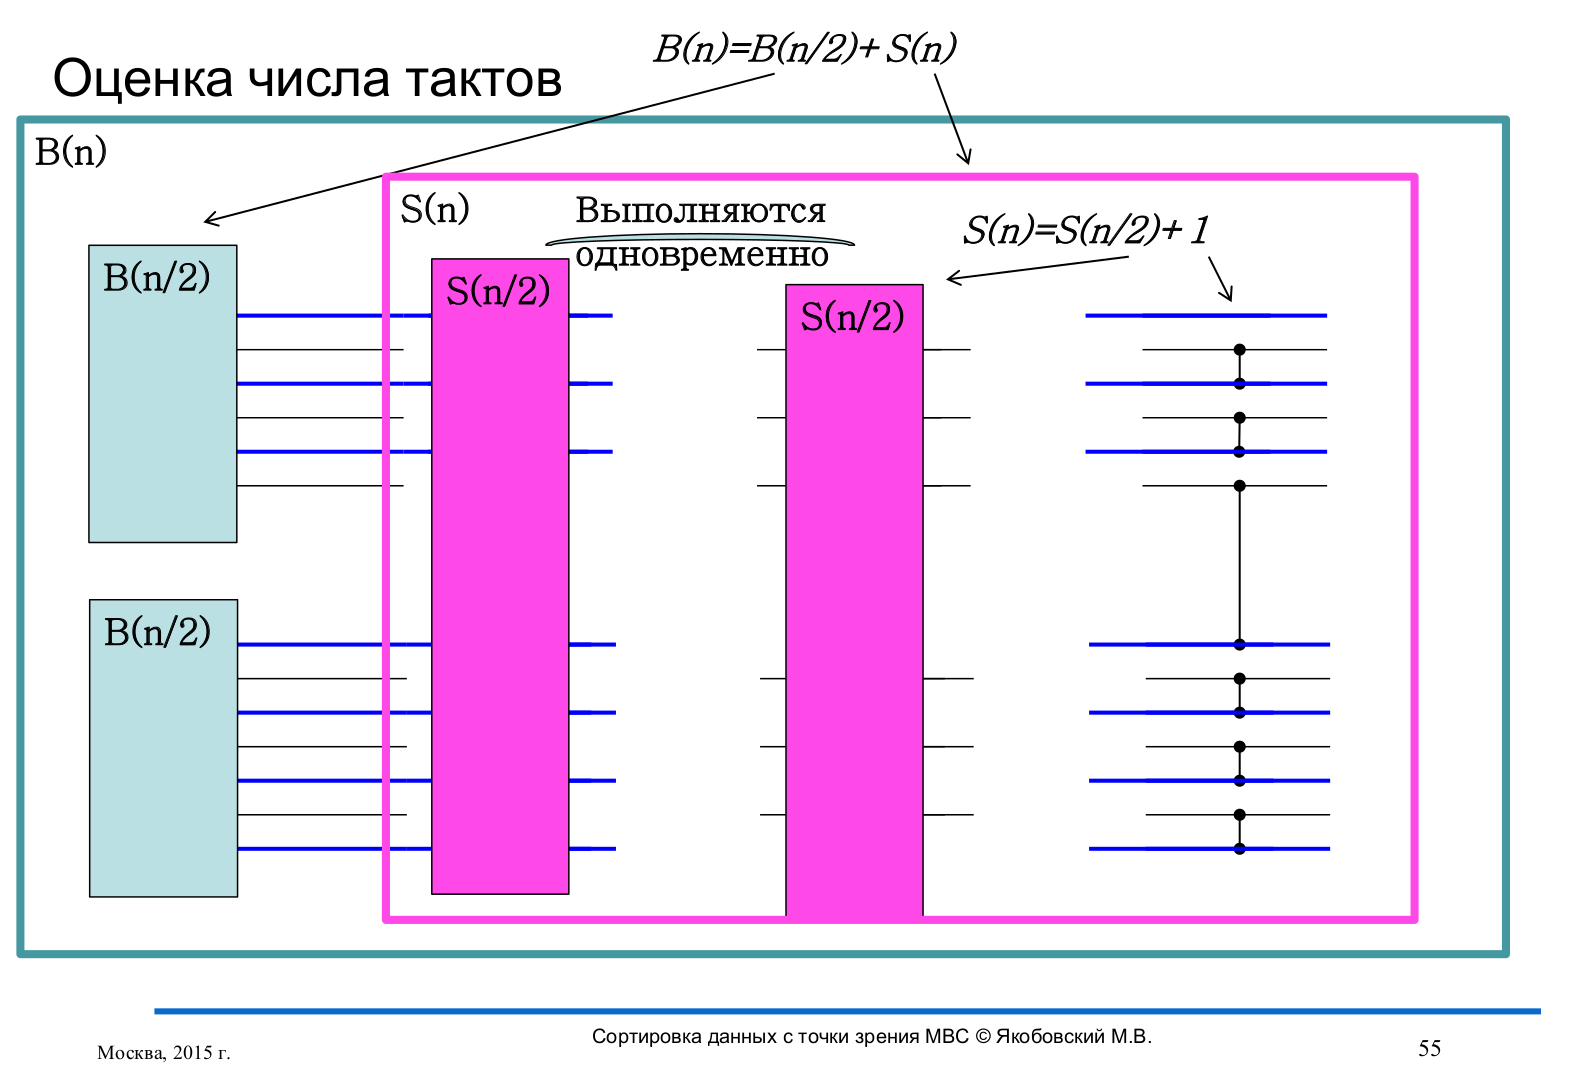
\includegraphics[scale=0.4]{tacts}
	\caption{Сортировка Бэтчера}
\end{figure}

Получим систему уравнений:
\begin{equation*}
B(p) = B \left( \frac{p}{2} \right) + S(p)
\end{equation*}
\begin{equation*}
S(p) = S \left( \frac{p}{2} \right) + 1.
\end{equation*}

Зная, что $B(2) = 1$, $S(2) = 1$, получим выражения, определяющие задержку сети:
\begin{equation*}
S(p) = \log_2 p
\end{equation*}
\begin{equation*}
B(p) = \frac{\log_2 p \left( \log_2 p + 1 \right)}{2}
\end{equation*}

Обозначая этими же буквами количества компараторов, получим следующую систему:
\begin{equation*}
B(p) = 2B \left( \frac{p}{2} \right) + S(p)
\end{equation*}
\begin{equation*}
S(p) = 2S \left( \frac{p}{2} \right) + \frac{p}{2} - 1.
\end{equation*}

Зная, что $B(2) = 1$, $S(2) = 1$, получим выражения, определяющие число компараторов в сети:
\begin{equation*}
S(p) = \frac{p}{2} \log_2 \frac{p}{2} + 1
\end{equation*}
\begin{equation*}
B(p) = \frac{p \log_2 p \left( \log_2 p - 1 \right)}{4} + p-1
\end{equation*}

\section{Алгоритм проверки}
Проверим корректность сети сортировки для $1 \leq n \leq 24$.
Будем опираться на принцип нулей и единиц: если сеть размера $n$ правильно сортирует всевозможные последовательности из 0 и 1 длины $n$, то она правильно сортирует последовательность любых чисел длины $n$. Разумеется, такая проверка не гарантирует, что сеть работает правильно при других размерах ($n>24$). Однако эта проверка есть необходимое условие корректности сети (а при $1<=n<=24$ ещё и достаточное).

Алгоритм выглядит крайне просто:
\begin{itemize}
\item[0] $n=1$
\item[1] создаём сеть сортировки размера $n$ (записываем последовательность компараторов в файл, например),
\item[2] сортируем все последовательности из 0 и 1 длины $n$ этой сетью и проверяем корректность сортировки,
\item[3] Если $n=24$, завершаем программу. Иначе $n += 1$ и переходим к шагу 1.
\end{itemize}

Единственный вопрос --- как грамотно создать все такие последовательности длины $n$. Очевидно, их будет ровно $2^n$ штук, причём их можно рассматривать как двоичную запись чисел от $0$ до $2^n-1$. Именно: перебираем числа от $0$ до $2^n-1$, получаем их бинарное представление в $n$ битах и сортируем это представление.

Код на языке Си, создающий представление $v$ длиной $n$ из числа $value$:
\begin{lstlisting}
void fillin(int *v, int n, int value)
{
    for(int i=n-1; i>=0; i-=1)
    {
        v[i] = value & 1;
        value = value >> 1;
    }
}
\end{lstlisting}

\end{document}\grid
